\begin{figure}[htbp]
  \centering
  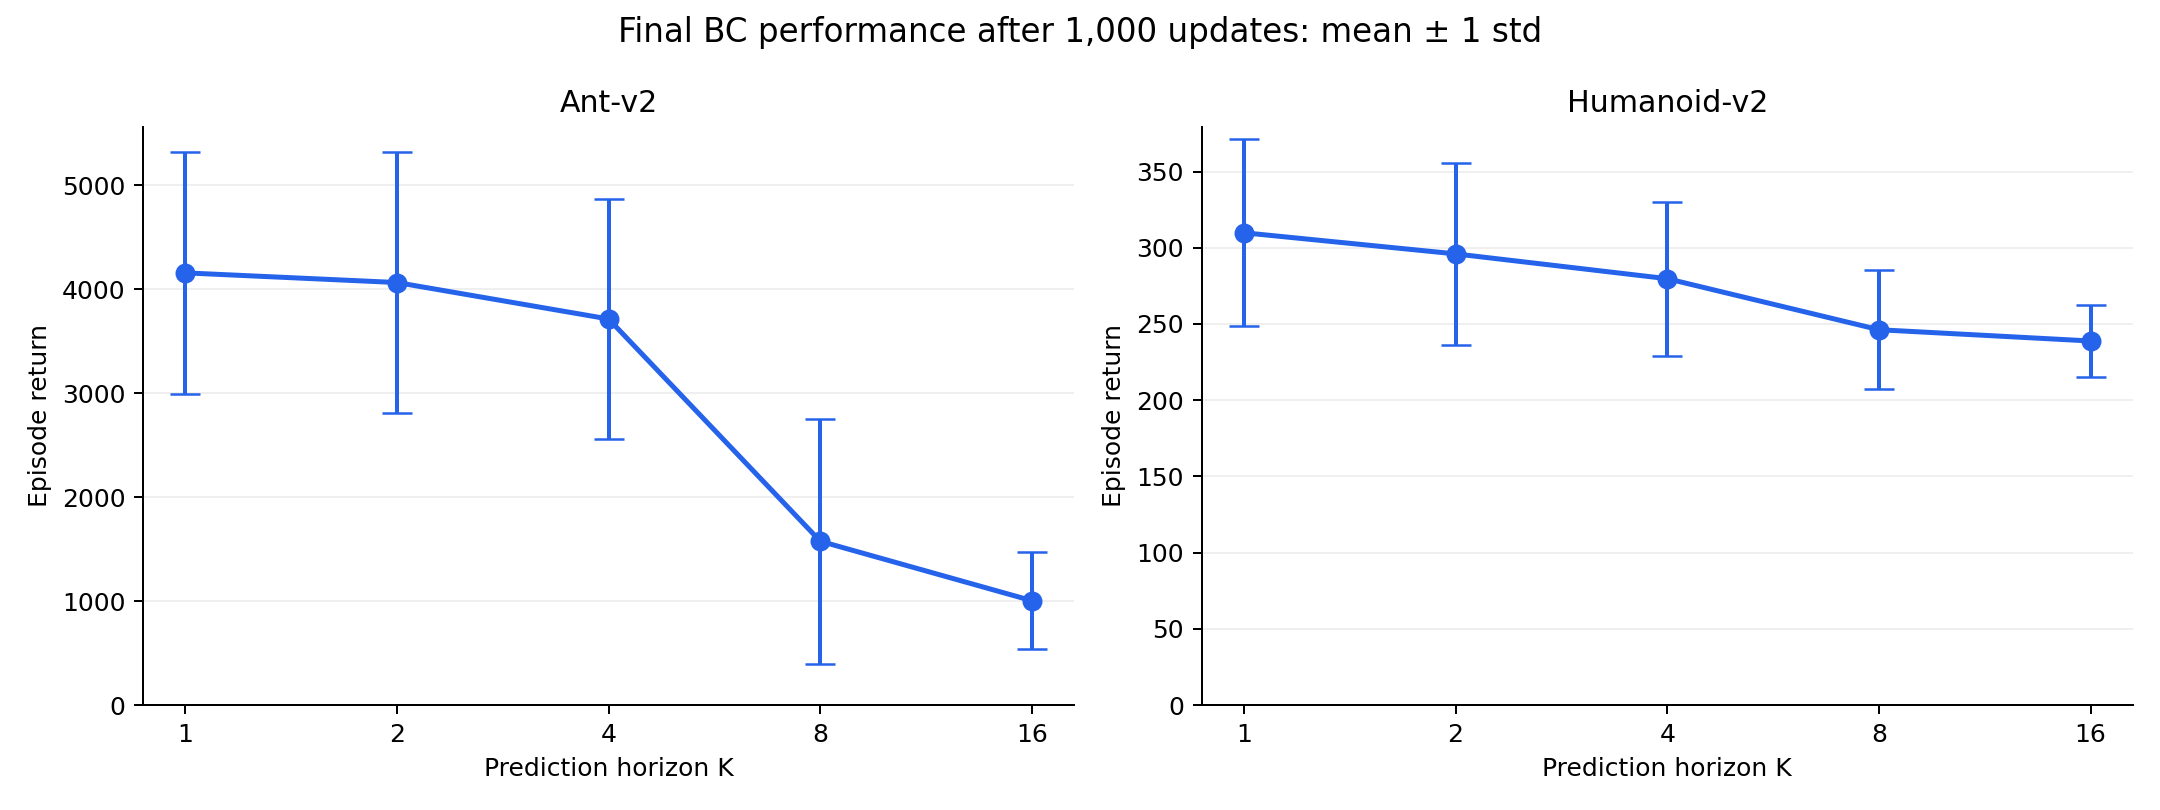
\includegraphics[width=\linewidth]{../results/action_chunks/main/figure1.png}
  \caption{Future-action prediction as auxiliary supervision for closed-loop BC on Ant-v2 and Humanoid-v2. Hypothesis: moderate prediction horizons improve imitation, while large horizons may degrade it. We vary only the action-prediction horizon $K\in\{1,2,4,8,16\}$; every step executes only the first prediction and replans from the new observation. All conditions use the same two expert trajectories (2,000 starting observations), 3 hidden layers of 64 tanh units, Adam with learning rate 0.005, 1000 updates, minibatches of 100, and training seeds [1, 2, 3]. Missing future targets are masked at episode boundaries; the output layer grows with $K$. Each trained policy is evaluated on at least 5 complete rollouts and 5000 steps, with a 1000-step episode limit and matched reset-seed schedules across horizons. Blue points and error bars show mean and population standard deviation of episode returns with equal weight per training seed after the final training update. Ant-v2: none of $K$=2,4,8 exceeded the $K$=1 aggregate mean. Humanoid-v2: none of $K$=2,4,8 exceeded the $K$=1 aggregate mean. The hypothesized moderate-horizon benefit was not supported under this training budget. These limited-seed observations do not establish statistical significance or isolate representation quality from output-head size and optimization effects.}
  \label{fig:p4}
\end{figure}
